\documentclass[conference]{IEEEtran}
%\renewcommand{\thesubsection}{\thesection.\alph{subsection}}

%\addtolength{\oddsidemargin}{-.875in}
%\addtolength{\evensidemargin}{-.875in}
%\addtolength{\textwidth}{1.75in}
%\addtolength{\topmargin}{-.875in}
%\addtolength{\textheight}{1.75in}
	
\usepackage{bm}
\usepackage{amsmath}
\usepackage{amssymb}
\usepackage{tikz}
\usetikzlibrary{automata,positioning}
\usepackage{url}
\usepackage{float}
\usepackage{setspace}
\usepackage{filecontents,lipsum}
\usepackage[noadjust]{cite}

\begin{document}
%\raggedright
%\doublespacing

\title{Week 3 Journal}
\author{Rodger Byrd}
\maketitle


\section{Topic Map}
For my area I'm looking at Anti-Patterns in code, these are also known as code smells. I've also seen them referred to as Atoms of Confusion and nano patterrns. My topic map is included below in figure \ref{fig:TM}. My thoughts on gaps are some method to demonstrate the found anti-patterns are valid. Also, there seems to be a gap in how to fix anti-patterns and code smells. I've also included my notes on creating the Topic map in Figure \ref{fig:TN}.
\begin{figure*}
  \centerline{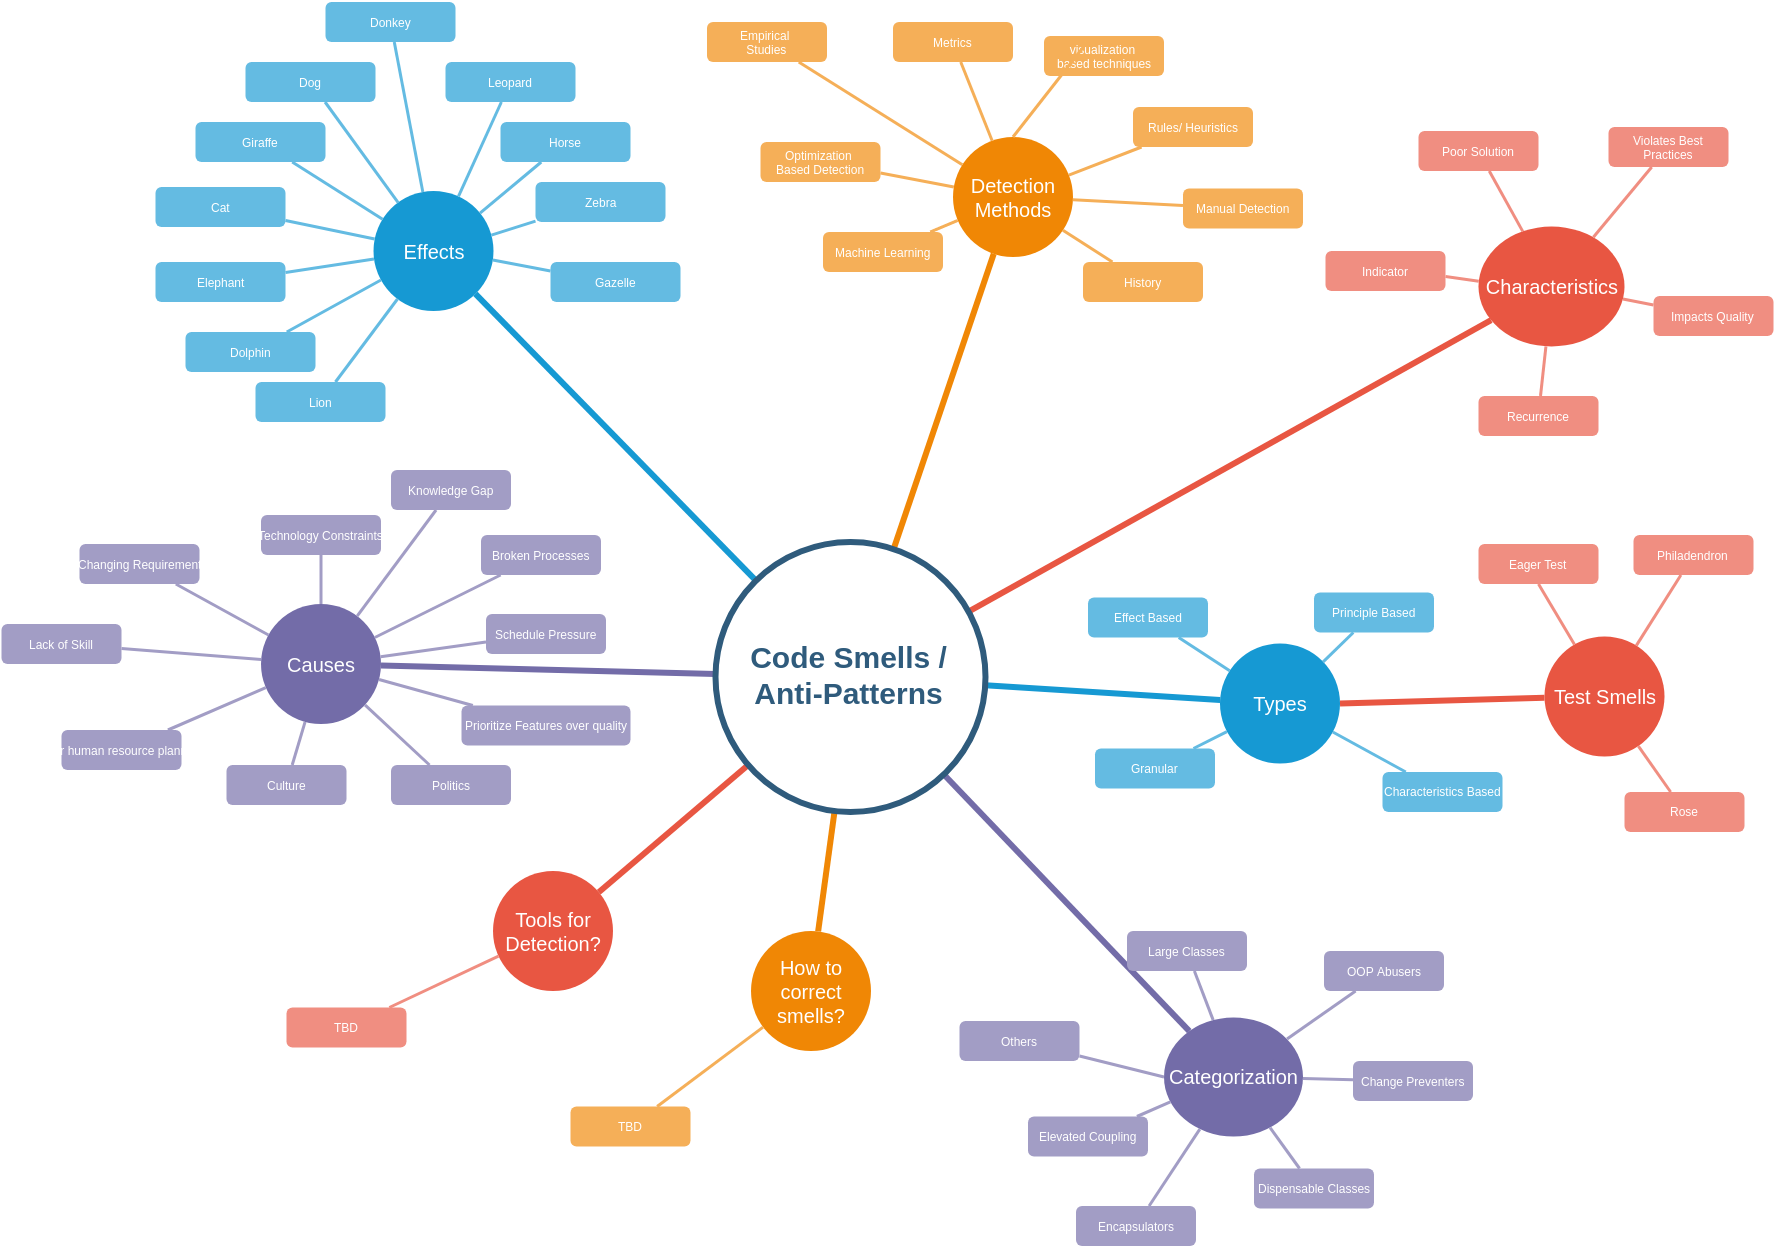
\includegraphics[width=\textwidth]{codesmells.png}}
  \caption{TopicMap}
  \label{fig:TM}
\end{figure*} 

\begin{figure*}
  \centerline{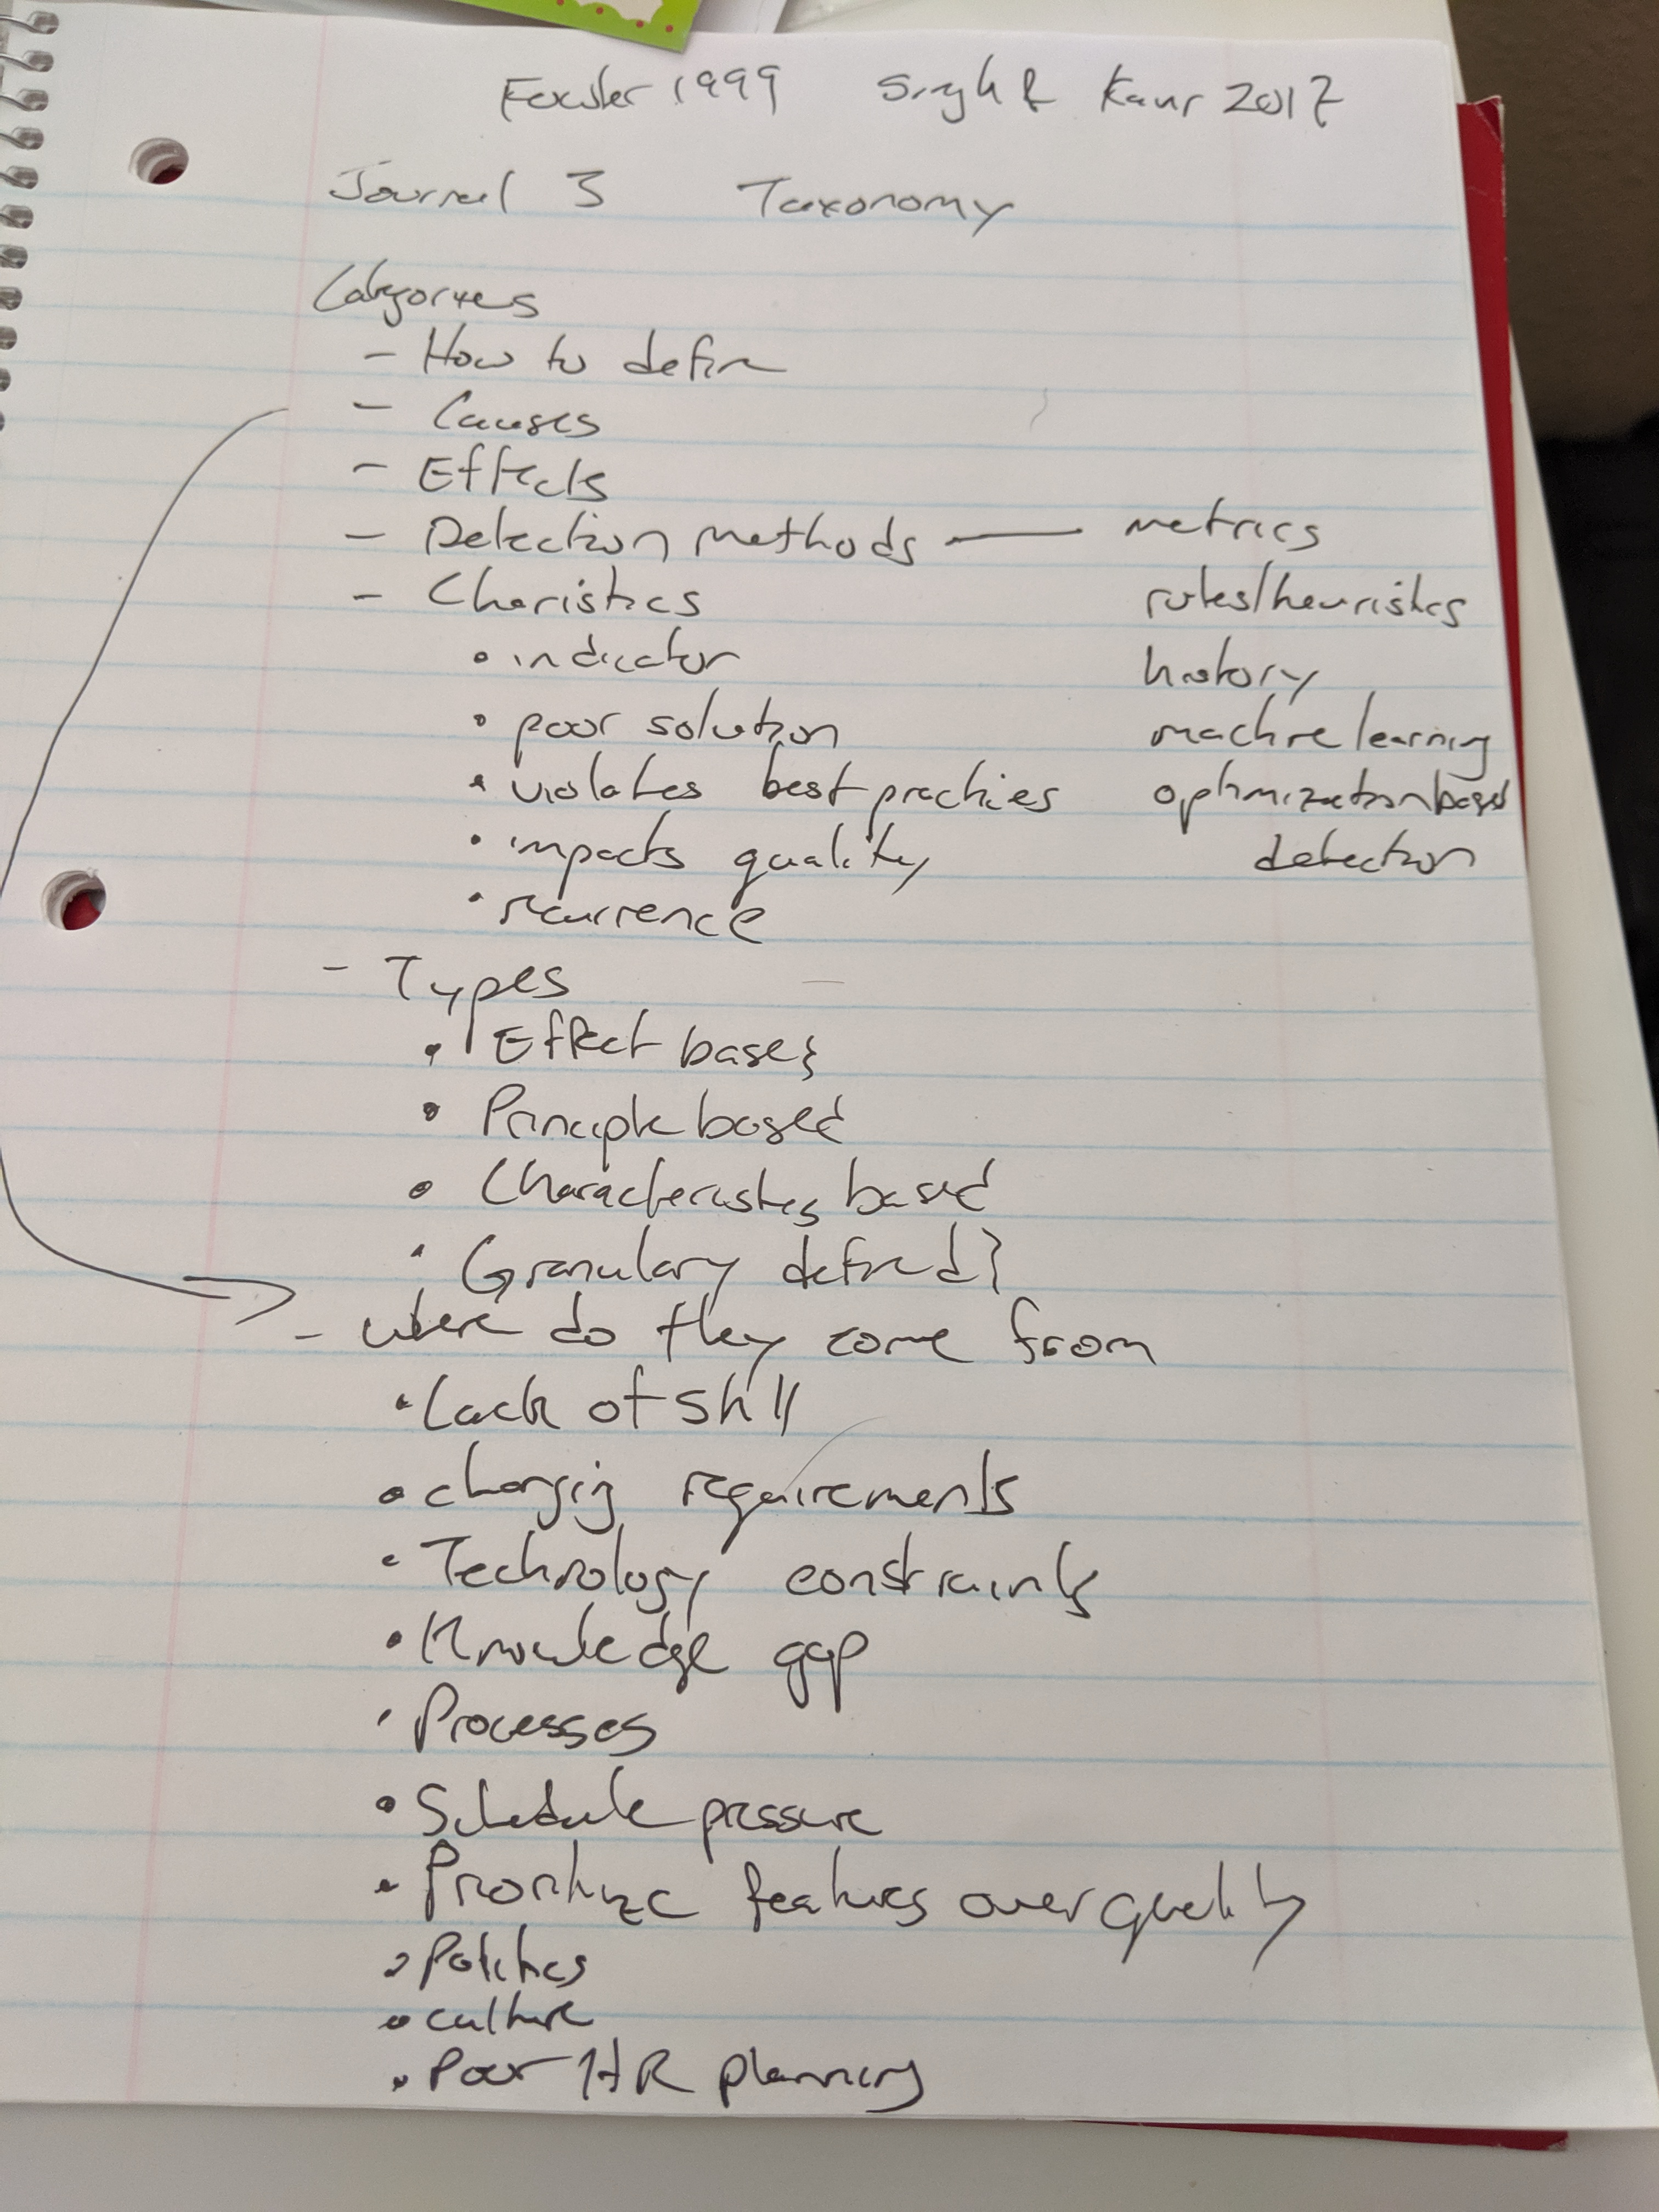
\includegraphics[width=\textwidth]{taxonomy_notes.jpg}}
  \caption{TopicMap}
  \label{fig:TN}
\end{figure*} 
\section{Notes on Survey Papers, }
For my first detailed read I chose a paper called  \textit{A survey on software smells} \cite{sharma_survey_2018}.
The following are my raw notes for this paper.

Kent Beck coined the term code smell, I should look at this paper.
Contains some ideas for topic map in abstract.
Figure 1 in paper has a pretty detailed topic map.
Interesting for comparison.
Table 4 code smells.
Interesting section on whether anti-patterns and smells synonyms, doesn't seem to be consensus. Some papers yes, some no.
Smell indicator of problem, anti pattern definitive problem.
Current detection methods cause too many false positives?
This wasn't as good as the first two papers, they did a very good job of summarizing the current research. This one talked way too much about how they did their analysis instead of the results.


For my next detailed read I chose a paper called  \textit{A systematic literature review: Refactoring for disclosing code smells in object oriented software} \cite{singh_systematic_2018}. 
The following are my raw notes for this paper.

Refers to code smells and anti-patterns interchangeably.
Related work is basically a background.
Included 238 of an initial 1053 articles.
Wow, that is a ton of papers.
The papers they drew from were on the following topics: Refactoring, anti-patterns, code smells, Object Oriented Design and refactoring, fault tolerance and OOD, SW Metrics and anti-patterns, anti-patterns in cross company projects.
Provide a lot of detail on the detection methods
Interesting to show charts based on the publisher, Conference proceedings and IEEE were top sources.


For my next detailed read I chose a paper called  \textit{Smells in software test code: A survey of knowledge in industry and academia} \cite{garousi_smells_2018}. 
The following are my raw notes for this paper.

Interesting variation on the idea of anti pattern: "test smells".
Poorly designed tests.
Really weird figures in this paper, copy paste screenshots out of spreadsheet and websites like google.
Just make a table!
They are missing the visualization, they are showing tons of tables instead of the results of the research.
Missing the analysis?


The files for this latex document are in the github repository located at \path{https://github.com/rodger79/CS6000}

Papers that were scanned and trashed are referenced in the bibliography below. 
\nocite{*}
\clearpage


\bibliographystyle{IEEEtran}
\bibliography{references}


\end{document}